\section{Planification Initiale}

\subsection{Jalons}

\subsubsection{Jalons fixées par l'INSA}

Ci-dessous les dates fixées par l'INSA, qui ont fait office de jalons pendant toute la durée du projet.\\

\begin{tabular}{|l|l|}
\hline
  Date &
  Production \\
\hline
  12 février &
  Rapport de conception logicielle  \\
\hline
  2 avril &
  Page HTML  \\
\hline
  26 mai &
  Rapport Final/Annexes + Bilan Planification \\
\hline
  28 mai &
  Documentation en Ligne VF \\
\hline
\end{tabular}


\subsubsection{Jalons internes}
Dans le but de gérer notre avancement dans le temps et d'obtenir des retours de la part de Kerpape, nous nous étions fixé des jalons \enquote{internes}.
Ceux-ci consistaient en un certain nombre de versions intermédiaires du logiciel à livrer, versions plus ou moins éloignées les unes des autres.
Nous avions fixé des niveaux de fonctionnalité pour chaque version, par exemple, la version n°3 devait intégrer les collisions dans la scène entre l'utilisateur et les divers objets.\\

\begin{tabular}{|l|l|}
\hline
  Date &
  Production \\
\hline
  9 janvier &
  Version PC \textnumero2 \\
\hline
  9 février &
  Version PC \textnumero3 \\
\hline
  9 mars &
  Version PC \textnumero4 \\
\hline
  9 avril &
  Version PC \textnumero5 \\
\hline
\end{tabular}\\

\subsection{Méthode de travail}

Les jalons imposés, les fonctionnalités prévues en avance et les seuils d'acceptation/validation que nous nous étions fixés nous ont naturellement conduits à travailler en suivant un cycle en V.
Les dates de rendus de rapports à l'INSA ont bien sûr fait office de jalons dans ce cycle en V.
En revanche, nos jalons internes (livrables pour Kerpape) ont ajouté à ce cycle en V une coloration agile, composée de retours et corrections.

Un autre aspect de cette coloration agile est du refactoring régulier.
En effet, que ce soit dans les scripts ou dans la hiérarchie du projet Unity, ou encore dans l'arbre de la scène, nous avions prévu que réorganiser les fichiers, la hiérarchie des objets ou le code nous prendrait un certain temps.

\subsection{Estimations}

Pour réaliser la solution pour Kerpape nous avions fait une estimation du nombre d'heures nécessaires.
Nos estimations étaient basées sur nos expériences personnelles, venant d'autres projets, et de divers retours d'expérience.
Nous avions estimé à environ 600 heures de travail les fonctionnalités restantes après le mois de février.
Dans ce planning nous avions compté les week-end, les séances de projets, les vacances mais pas les semaines de partiels ni les semaines de révisions.

\subsubsection{Chronologie du projet}
Cette vue (cf.\textsc{figure~\ref{fig:timeline}}) est la plus synthétique que nous ayons réalisée, elle donne une vue d'ensemble du projet ne comprenant que les plus grandes étapes. 
\begin{figure}[h]
	\centering
	\caption{Chronologie générale}
		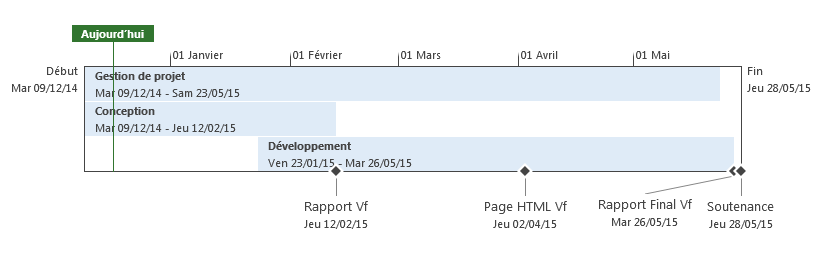
\includegraphics[width=\textwidth]{8-BilanPlanification/img/timeline.PNG}
	\label{fig:timeline}
\end{figure}

\subsubsection{Temps de travail cumulé}
Le temps de travail cumulé (cf.\textsc{figure~\ref{fig:avancement}}) restant est assez équilibré tout au long du projet avec toutefois quelques variations brusques autour des jalons précédemment définis.
Ces variations sont liées au fait que nous avons dégagé plus de temps autour des jalons en cas de problèmes. 

\begin{figure}[h]
	\centering
	\caption{Temps de travail cumulé restant}
		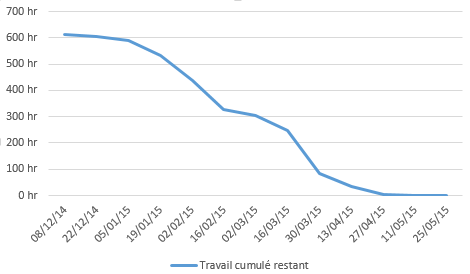
\includegraphics[width=\textwidth]{8-BilanPlanification/img/avancement.PNG}
	\label{fig:avancement}
\end{figure}